
\documentclass[10pt]{beamer}
\usepackage{amsmath}
\usepackage{mathtools}
\usepackage{multimedia}
\usepackage{hyperref}


\usefonttheme{professionalfonts} % using non standard fonts for beamer
\usefonttheme{serif} % default family is serif
%\documentclass[12pt]{beamerthemeSam.sty}
\usepackage{epsf}
%\usepackage{pstricks}
%\usepackage[orientation=portrait,size=A4]{beamerposter}
\geometry{paperwidth=160mm,paperheight=120mm}
%DT favorite definitions
\def\LL{\left\langle}	% left angle bracket
\def\RR{\right\rangle}	% right angle bracket
\def\LP{\left(}		% left parenthesis
\def\RP{\right)}	% right parenthesis
\def\LB{\left\{}	% left curly bracket
\def\RB{\right\}}	% right curly bracket
\def\PAR#1#2{ {{\partial #1}\over{\partial #2}} }
\def\PARTWO#1#2{ {{\partial^2 #1}\over{\partial #2}^2} }
\def\PARTWOMIX#1#2#3{ {{\partial^2 #1}\over{\partial #2 \partial #3}} }

\def\rightpartial{{\overrightarrow\partial}}
\def\leftpartial{{\overleftarrow\partial}}
\def\diffpartial{\buildrel\leftrightarrow\over\partial}

\def\BS{\bigskip}
\def\BC{\begin{center}}
\def\EC{\end{center}}
\def\BN{\begin{enumerate}}
\def\EN{\end{enumerate}}
\def\BI{\begin{itemize}}
\def\EI{\end{itemize}}
\def\BE{\begin{displaymath}}
\def\EE{\end{displaymath}}
\def\BEA{\begin{eqnarray*}}
\def\EEA{\end{eqnarray*}}
\def\BNEA{\begin{eqnarray}}
\def\ENEA{\end{eqnarray}}
\def\EL{\nonumber\\}

\newcommand{\etal}{{\it et al.}}
\newcommand{\gbeta}{6/g^2}
\newcommand{\la}[1]{\label{#1}}
\newcommand{\ie}{{\em i.e.\ }}
\newcommand{\eg}{{\em e.\,g.\ }}
\newcommand{\cf}{cf.\ }
\newcommand{\etc}{etc.\ }
\newcommand{\atantwo}{{\rm atan2}}
\newcommand{\Tr}{{\rm Tr}}
\newcommand{\dt}{\Delta t}
\newcommand{\op}{{\cal O}}
\newcommand{\msbar}{{\overline{\rm MS}}}
\def\chpt{\raise0.4ex\hbox{$\chi$}PT}
\def\schpt{S\raise0.4ex\hbox{$\chi$}PT}
\def\MeV{{\rm Me\!V}}
\def\GeV{{\rm Ge\!V}}

%AB: my color definitions
%\definecolor{mygarnet}{rgb}{0.445,0.184,0.215}
%\definecolor{mygold}{rgb}{0.848,0.848,0.098}
%\definecolor{myg2g}{rgb}{0.647,0.316,0.157}
\definecolor{A}{rgb}{1.0,0.3,0.3}
\definecolor{B}{rgb}{0.0,1.0,0.0}
\definecolor{C}{rgb}{1.0,1.0,0.0}
\definecolor{D}{rgb}{0.5,0.5,1.0}
\definecolor{E}{rgb}{0.7,0.7,0.7}
\definecolor{abtitlecolor}{rgb}{1.0,1.0,1.0}
\definecolor{absecondarycolor}{rgb}{0.0,0.416,0.804}
\definecolor{abprimarycolor}{rgb}{1.0,0.686,0.0}
\definecolor{Red}           {rgb}{1,0.4,0.4}
\definecolor{Yellow}           {rgb}{1,1,0.0}
\definecolor{Grey}          {cmyk}{.7,.7,.7,0}
\definecolor{Blue}          {cmyk}{1,1,0,0}
\definecolor{Green}         {cmyk}{1,0,1,0}
\definecolor{Brown}         {cmyk}{0,0.81,1,0.60}
\definecolor{Silver}        {rgb}{0.95,0.9,1.0}
\definecolor{Sky}           {rgb}{0.07,0.0,0.2}
\definecolor{Darkbrown}     {rgb}{0.4,0.3,0.2}
\definecolor{40Gray}        {rgb}{0.4,0.4,0.5}
\usetheme{Madrid}


\setbeamercolor{normal text}{fg=Silver,bg=Sky}

%AB: redefinition of beamer colors
%\setbeamercolor{palette tertiary}{fg=white,bg=mygarnet}
%\setbeamercolor{palette secondary}{fg=white,bg=myg2g}
%\setbeamercolor{palette primary}{fg=black,bg=mygold}
\setbeamercolor{title}{fg=abtitlecolor}
\setbeamercolor{frametitle}{fg=abtitlecolor}
\setbeamercolor{palette tertiary}{fg=white,bg=Darkbrown}
\setbeamercolor{palette secondary}{fg=white,bg=absecondarycolor}
\setbeamercolor{palette primary}{fg=white,bg=40Gray}
\setbeamercolor{structure}{fg=abtitlecolor}

\setbeamerfont{section in toc}{series=\bfseries}

%AB: remove navigation icons
\beamertemplatenavigationsymbolsempty
\title[Astromechanics: gravity]{
  \textbf {Astromechanics: gravity}}


\author [Astronomy 101]{Astronomy 101\\Syracuse University, Fall 2021\\Walter Freeman}

\date{\today}

\begin{document}



\frame{\titlepage}

\frame{
\Large

\BC{\it ``Truth is ever to be found in simplicity, and not in the multiplicity and confusion of things."}\EC
\bigskip 
\large
\begin{flushright}--Newton, {\it Rules for methodizing the Apocalypse} \\(n.b.: ``apocalypse'' also means ``revealing'')\end{flushright}


\bigskip
\bigskip
\bigskip
\bigskip
\bigskip
\Large
\BC{\it ``We are to admit no more causes of natural things than such as are both true and sufficient to explain their appearances.''}\EC
\bigskip
\large
\begin{flushright}--Newton, {\it Philosophiae Naturalis Principia Mathematica} \\(Mathematical Principles of Natural Philosophy)\end{flushright}


}
\frame{

\Huge\BC\it
``What is a neutron star?''
\EC
\Large
\begin{flushright}--Paritosh, AST101 student\end{flushright}

}

\frame{
	\Large
	A neutron star is what happens when gravity crushes dead stars.
	\large
	\BI
	
	\item Stars have a huge mass, and thus have huge amounts of gravity
	\item While they burn they are supported against that gravity by the heat coming from their cores
	\item Once they run out of fuel, their cores collapse.
	
	\BS\BS\BS
	
	\item Quantum mechanics limits how tightly you can pack particles together. {\it ``Pauli exclusion principle''}
	\item Our Sun, when it dies, will be crushed by its own gravity into a ball of carbon atoms -- a white dwarf.
	\item The quantum exclusion principle, acting on the electrons in the carbon, holds it up.
	\item It will sit there forever, slowly cooling down, unless something else hits it.
	
	\BS
	\EI
	
}

\frame{
	\Large
	A neutron star is what happens when gravity crushes dead stars.
	\large
	\BI

\item The exclusion principle, holding up the white dwarf left behind on the Sun, acts more weakly on heavy particles.

\BS

\item Atoms are made of three kinds of particles...
\pause
\BI
\item Positive protons (heavy!)
\item Neutral neutrons (also heavy!)
\item Negative electrons (2000 times lighter!)
\EI
\pause
\BS

\item If we could get rid of those pesky electrons, we could crush them even tighter!

\pause

\item If a star is massive enough, its gravity is strong enough to crush positive protons and negative electrons together to make neutrons.

\BS

\item These can be packed incredibly tightly, since the exclusion principle is weaker.

\item They are a hundred million billion times denser than water! ($10^{17}$)

\EI
}

\frame{

\Large

Today we're learning about gravity.

\BS

We'll see that gravity is stronger for objects with larger mass, and also stronger if you get closer. 

\BS

A neutron star has an extremely large mass (a little more than the Sun), and since it is so small, you can get very close to it...

\BS\BS\pause

... so there should be {\it extreme gravity} on its surface.

\BS\BS\BS

It's about 500 billion times as strong as Earth's!
}





\frame{\frametitle{\textbf{Kepler's laws, summarized}}
\Large
\BI
\item 1. Planets travel in elliptical orbits, with the Sun at one focus
\item 2. The line going from the Sun to the planet sweeps out equal areas in equal times
\item 3. The time that a planet takes to go around the Sun increases as the 3/2 power of the long axis of the ellipse.
\EI
}

\frame{\frametitle{\textbf{Kepler's second law}}
\Large
\BC
The line from the Sun to the planet sweeps out equal areas in equal times.

\bigskip

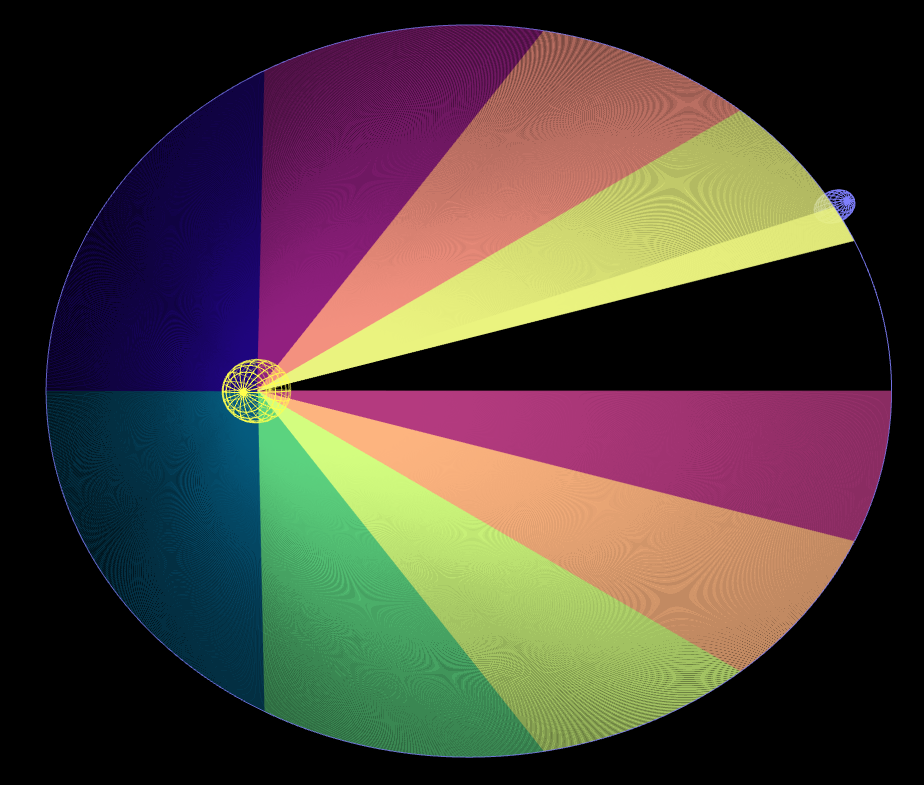
\includegraphics[width=0.5\textwidth]{equal-areas.png}

\bigskip
\bigskip

Each colored wedge has the {\it same area}, and the planet takes the {\it same time} to go through each.

\bigskip
\bigskip

This means that it moves {\it faster} when it's nearer the Sun.
\EC
}

\frame{\frametitle{\textbf{Kepler's Third Law}}

\Large
Kepler's third law of orbital motion says that the square of a planet's {\it orbital period} is proportional
to the cube of its {\it semimajor axis}.

\bigskip
\bigskip
\bigskip

Simply put: if a planet is further from the Sun, it takes longer to go around.

\bigskip
\bigskip
\bigskip

If the distance is doubled, the time required {\it more than doubles}.

\bigskip
\bigskip
\bigskip

Let's watch this...

}

\frame{
\Large
Saturn is about 10 AU from the Sun, while Uranus is about 20 AU from the Sun.

\bigskip
\bigskip

Saturn takes about 30 years to orbit the Sun. About how long does Uranus take?

\bigskip
\bigskip

\huge

\color{A}A: About 30 years\\
\color{B}B: Between 30 and 60 years \\ 
\color{C}C: More than 60 years \\
\color{D}D: It depends on the masses of Uranus and Saturn \\
\pause
\color{E}E: I looked it up on Wikipedia...
}

\frame{
\BC
\Huge
Finish your exercises from last time and start on your homework.
\bigskip
\bigskip

\Large

Raise your hands if you have questions. After this, we will study gravity.
\EC
}

\frame{

\BC

\Huge 
Do you think Kepler's laws can apply to things besides planets? Why or why not?
\vspace{1in}

\Large

Talk about this with your neighbors. I'll call on some random people and ask for your thoughts in a minute.

\EC

}

\frame{\frametitle{\textbf{Asking what vs. asking why}}
	
	\Large
	
	Remember, Kepler only discovered {\it what} the planets' orbits looked like.
	
	\BS
	
	He desperately wanted to know {\it why} they moved in that way, but he never could figure it out.
	
	\BS
	
	It turns out that if we can understand {\it why}, we can understand some other things, too...

}


\frame{\frametitle{\textbf{Natural laws vs. their consequences}}
\Large
Obviously the world around us is very diverse. Some things in it look quite simple:

\BI
\item{The motion of the stars}
\item{The near-perfect-spheres of the planets and moons}
\item{The elliptical motions of the planets (?)}
\item{The colors in a rainbow}
\EI
\pause
\bigskip

Others, though, are maddeningly complex:

\BI
\item{Seismic waves and earthquakes}
\item{The colors in the Sun}
\item{The weather}
\item{The diversity of rocks on Earth}
\pause
\item{Even the simplest living things}
\pause
\item{... language, culture, music, art, and all the creations of humankind...}
\EI
}

\frame{\frametitle{\textbf{Elegance, revisited}}

\BC
\Large

The laws of the Universe are simple and elegant. 

The things the Universe builds out of them are often complex!

\bigskip
\bigskip
\bigskip
\EC
\begin{columns}
\column{0.5\textwidth}
\BC
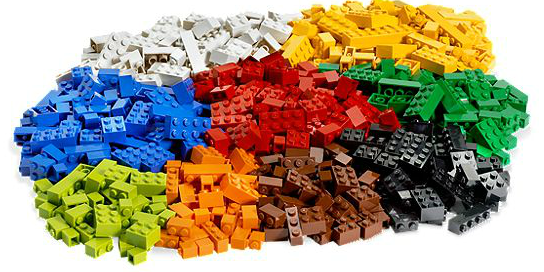
\includegraphics[width=0.8\textwidth]{lego-set.png}
\EC
\pause
\column{0.5\textwidth}
\BC
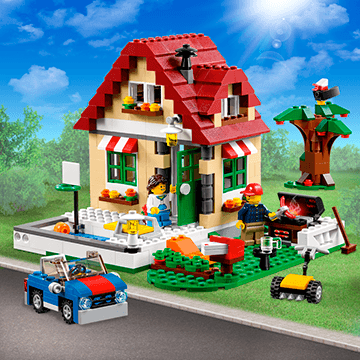
\includegraphics[width=0.8\textwidth]{lego-house.png}
\EC
\end{columns}
}



%\frame{\frametitle{\textbf{Natural laws vs. their consequences}}
%\large
%We've been doing science for a few hundred years, and we've noticed a pattern.
%
%\bigskip
%
%The Universe seems to operate according to a {\it very few} basic laws.
%\BI
%\item{There are {\it four forces} in nature, two of which are different manifestations of the same thing}
%\item{All these forces cause a few types of {\it elementary particles} to move around}
%\item{On a very small scale, this movement is governed by the laws of {\it quantum mechanics}}
%\item{On a bigger scale, QM turns into the much simpler {\it Newton's laws of motion}}
%\item{This movement takes place on the stage of {\it spacetime}}
%\EI
%
%\pause
%
%\bigskip
%
%When things are complicated (not simple and elegant) in Nature, it's because they are {\it complicated combinations} of pieces that are, themselves, simple -- pieces that obey simple laws.
%
%\pause
%\bigskip
%\bigskip
%
%... even us!
%}

\frame{\frametitle{\textbf{Isaac Newton}}

\begin{columns}
\column{0.4\textwidth}
\BC
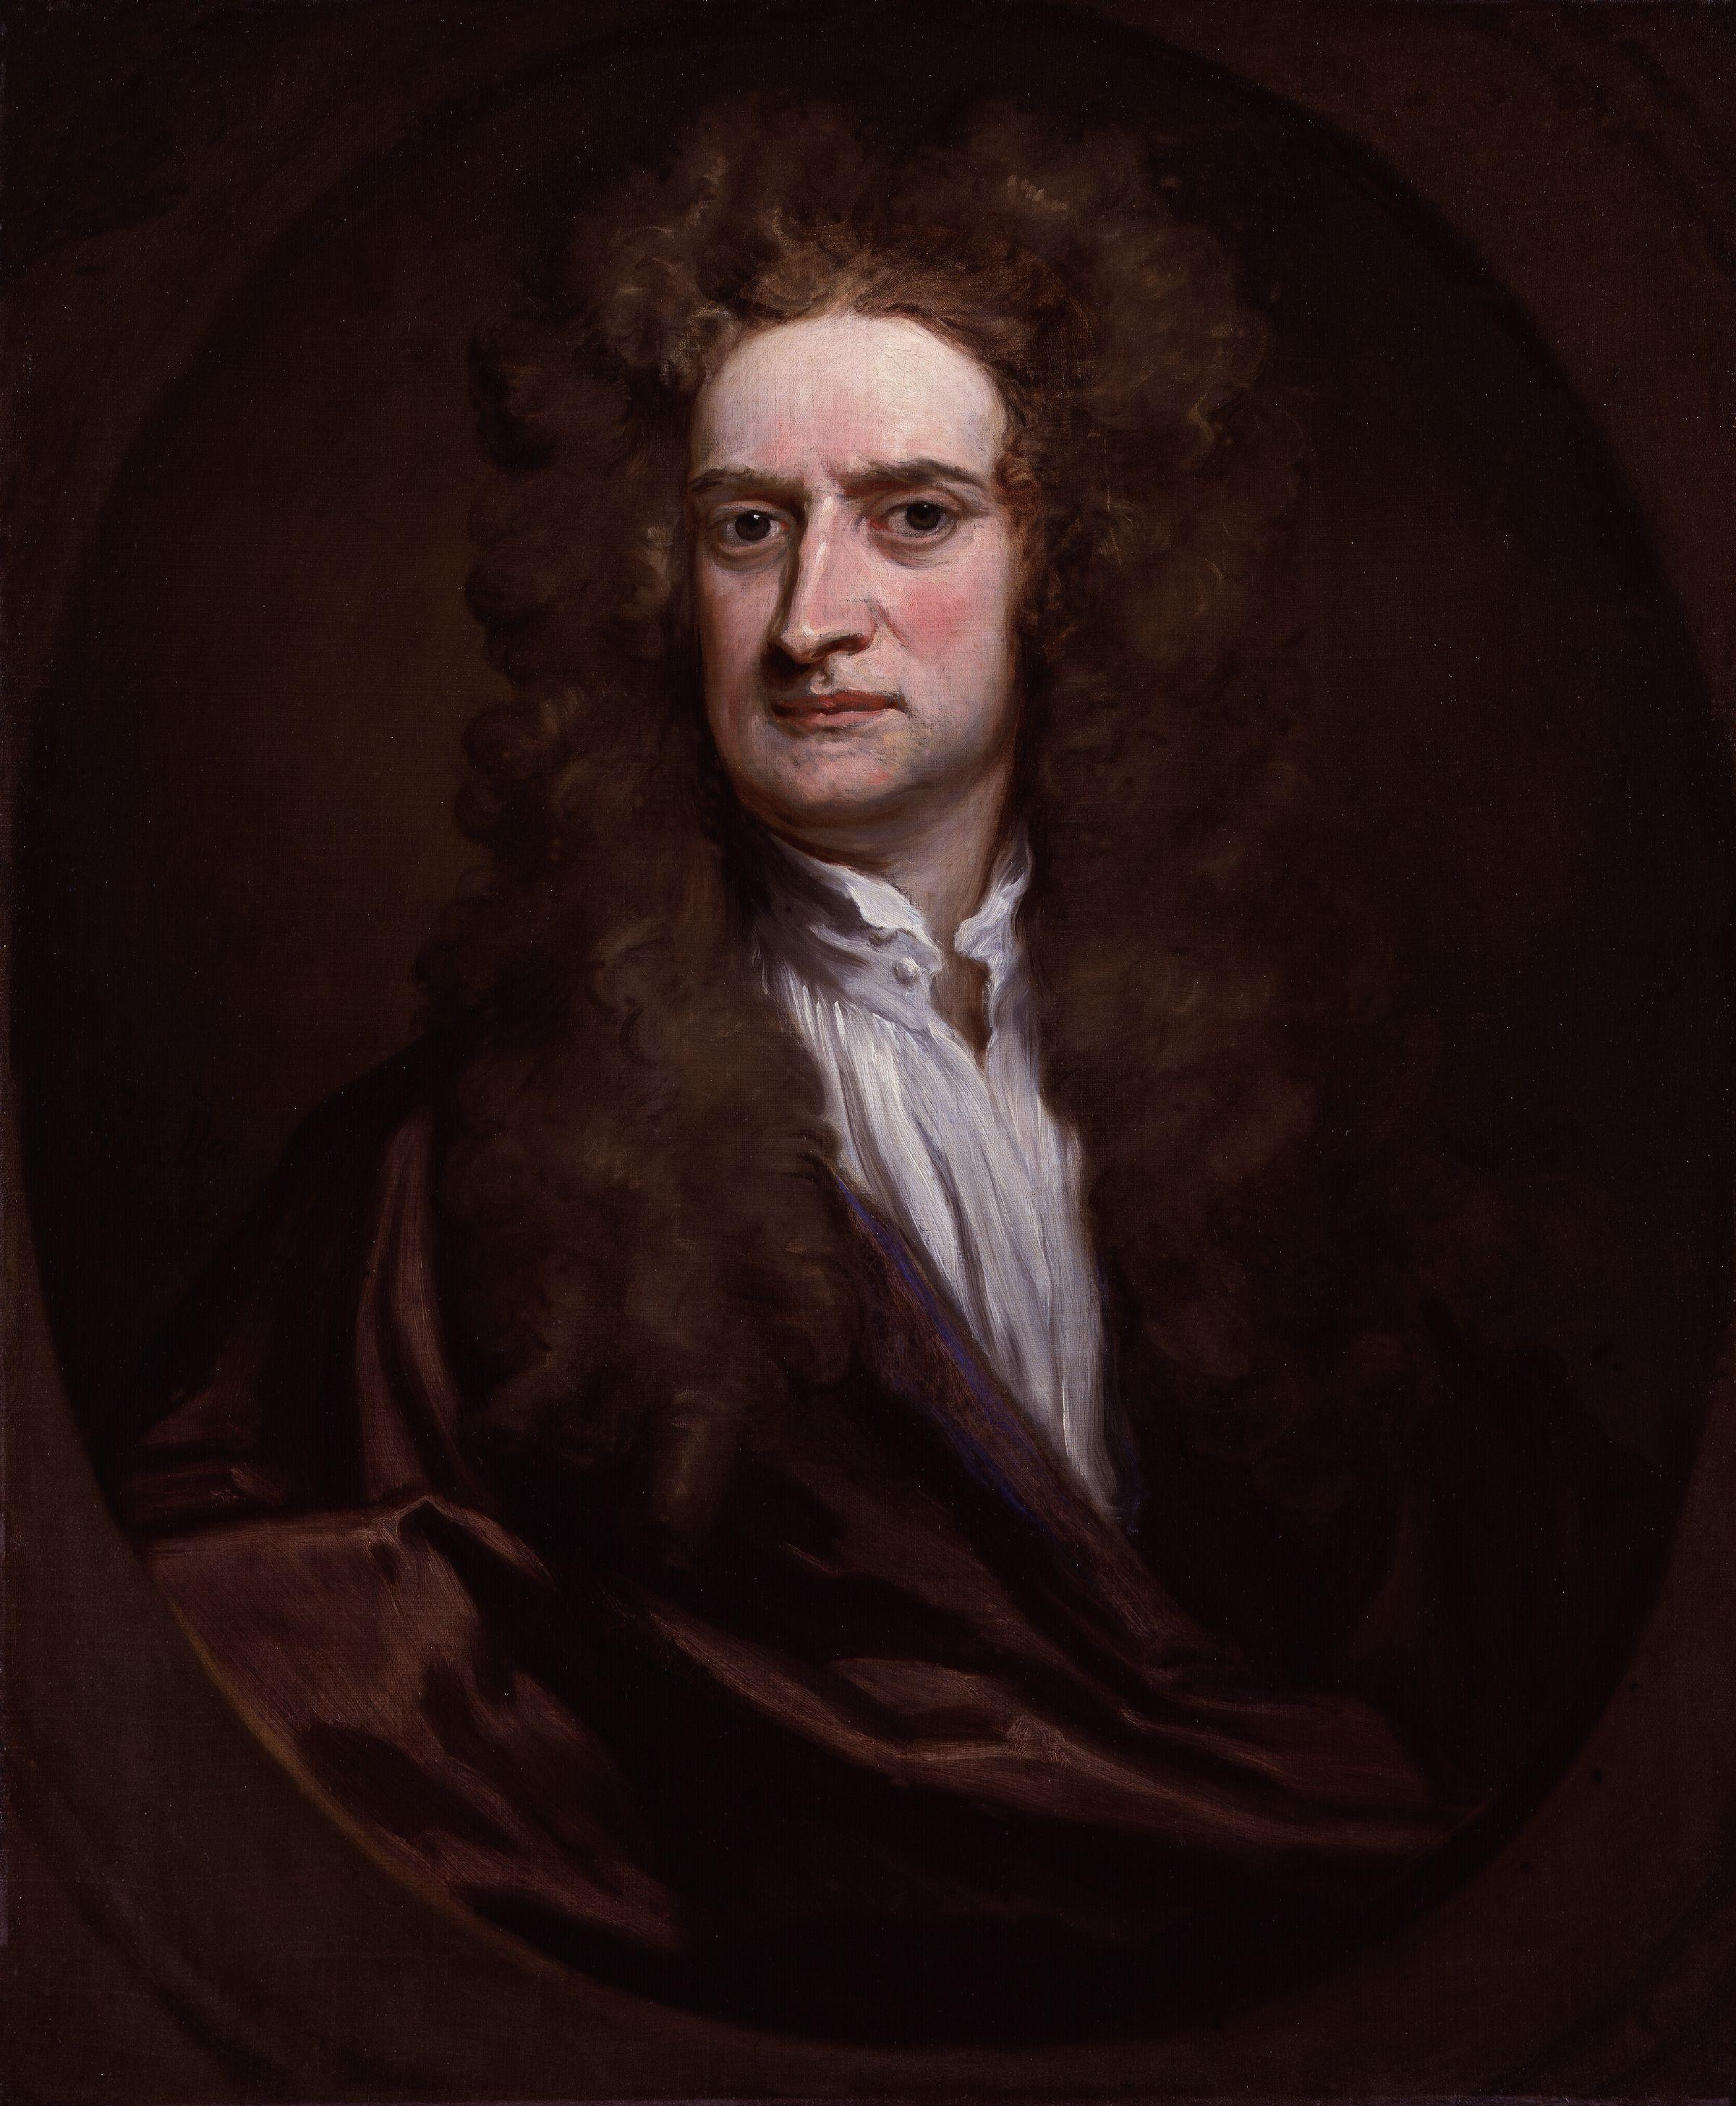
\includegraphics[width=\textwidth]{newton.jpg}
\EC
\column{0.6\textwidth}

\large
Isaac Newton (1642-1727 or 1726) finally figured out the laws that eluded Kepler.

\bigskip

He discovered...

\BI
\item{Forces cause objects to change their speed or direction of motion}
\item{Calculus -- the mathematics of changes}
\item{Gravity is such a force}
\item{The mathematical description of gravity}
\pause
\item{Principles of optics}
\item{The mathematics of cooling}
\item{... and much more}
\EI
\end{columns}
}


\frame{\frametitle{\textbf{Newton's biggest idea}}

\Huge
\BC

``Forces cause objects to accelerate''

\bigskip
\bigskip
\bigskip

$F=ma$

\bigskip
\bigskip
\bigskip

$F/m = a$

\bigskip
\bigskip
\bigskip

\Large

``The strength of a force, divided by the mass of the thing it acts on, gives that thing's acceleration''
\EC
}




\frame{\frametitle{\textbf{The law of gravity}}
\Large
Newton showed mathematically what Kepler suspected: that ``there is a force in the Earth that causes the Moon to move''.

\BS
That thing, of course, is gravity.
\BS\BS

Newton discovered:


\bigskip
\bigskip

All objects attract all other objects with a force that is:

\BI
\item{Proportional to the product of their masses}
\item{Inversely proportional to the distance between their centers, squared}
\EI

In symbols:

$$F = \frac{G m_1 m_2}{r^2}$$
}


\frame{
\BC
	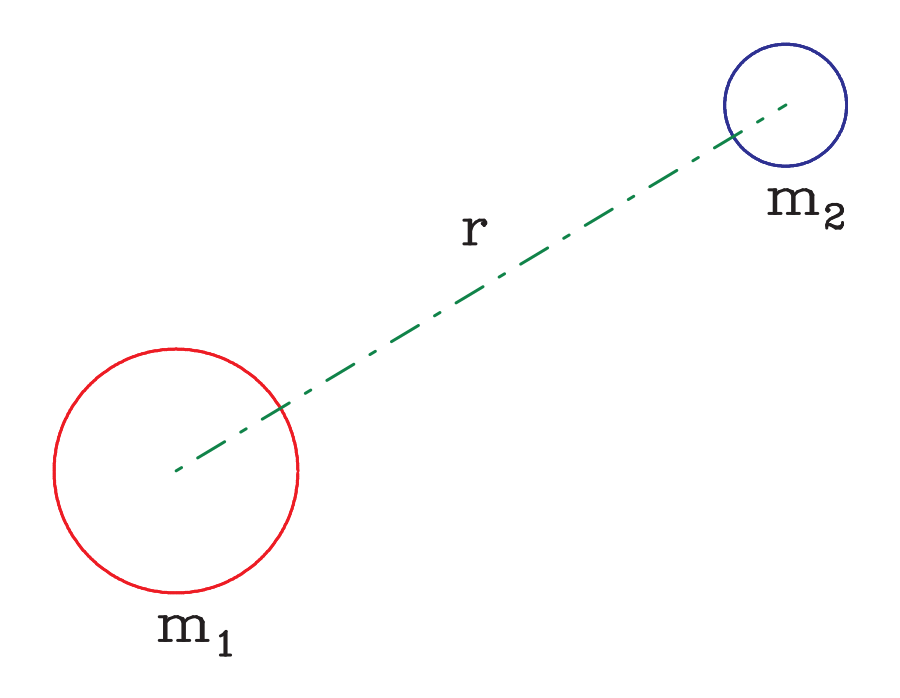
\includegraphics[width=0.65\textwidth]{law-gravity-crop.png}
	
	\Large
	
	\BS
	
	\Large
	
	The gravitational force between these two planets is $$F_g = \frac{G m_1 m_2}{r^2}.$$
\EC	
}

\frame{
	\begin{minipage}{0.5\textwidth}
		\hspace{0.15\textwidth}
			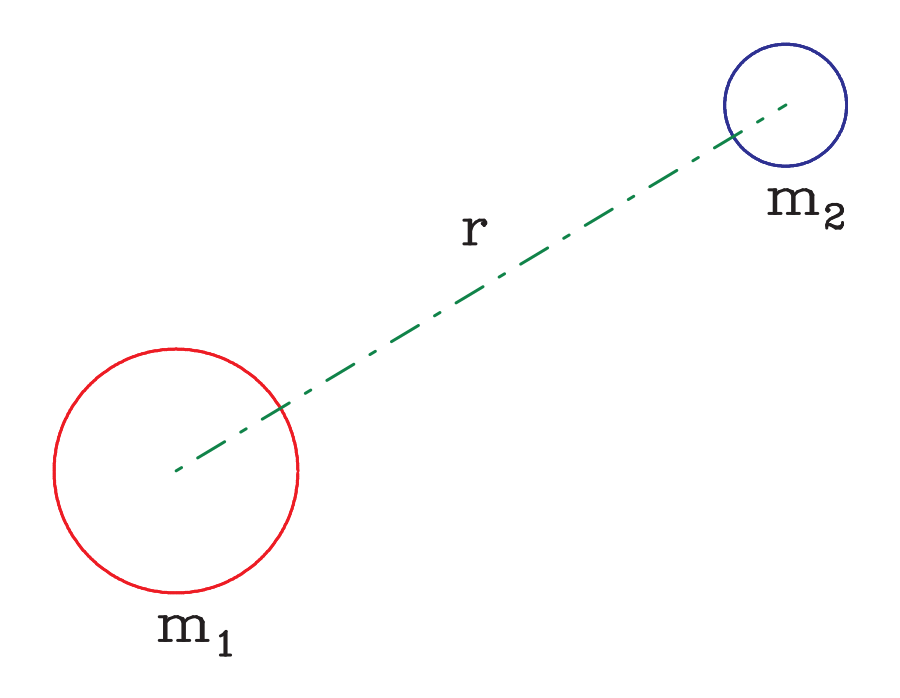
\includegraphics[width=0.7\textwidth]{law-gravity-crop.png}
	\end{minipage}
\begin{minipage}{0.49\textwidth}
	Here's the same diagram again. Suppose $m_1$ is a planet and $m_2$ its moon. As before the force on the moon is
	
	$$F_g = \frac{Gm_1m_2}{r^2}$$
	\end{minipage}

\Large

\BS\BS\BS

Suppose we make the planet twice as massive. How does the gravitational force on the moon change?

\BS\BS

\begin{minipage}{0.59\textwidth}
\color{A}A: It doesn't change

\color{B}B: It becomes twice as strong

\color{C}C: It becomes four times as strong

		\color{D}D: It becomes half as strong

\color{E}E: It becomes one-quarter as strong
\end{minipage}\pause
\begin{minipage}{0.4\textwidth}
	
	$$
	F_g = \frac{G{\color{Red}m_1}m_2}{r^2}
	$$
\end{minipage}
}

\frame{
	\begin{minipage}{0.5\textwidth}
		\hspace{0.15\textwidth}
		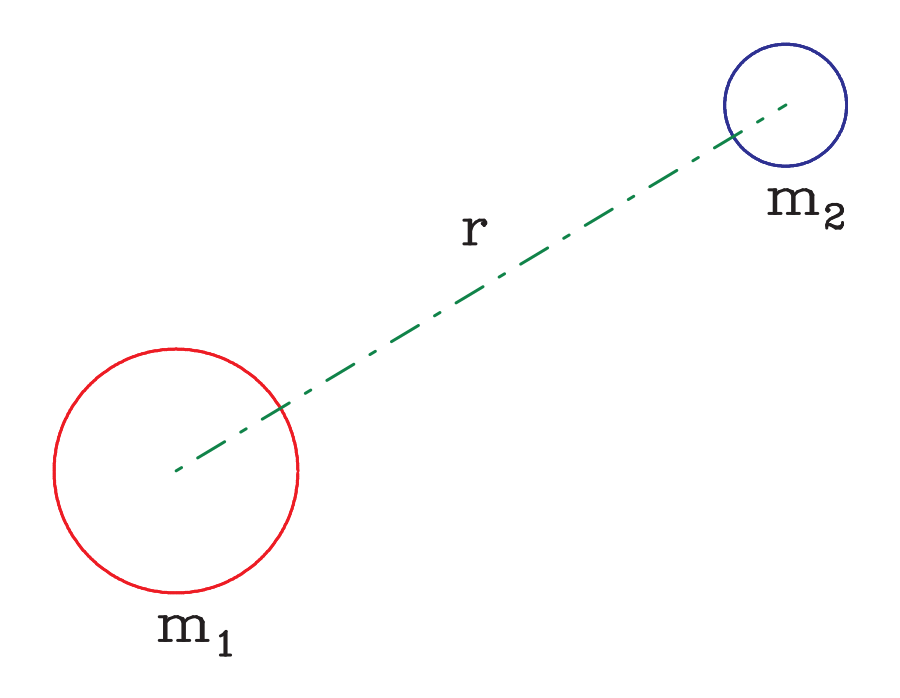
\includegraphics[width=0.7\textwidth]{law-gravity-crop.png}
	\end{minipage}
	\begin{minipage}{0.49\textwidth}
		Here's the same diagram again. Suppose $m_1$ is a planet and $m_2$ its moon. As before the force on the moon is
		
		$$F_g = \frac{Gm_1m_2}{r^2}$$
	\end{minipage}
	
	\Large
	
	\BS\BS\BS
	
	Suppose we make the planet twice as massive. How does the gravitational force on the moon change?
	
	\BS\BS
	
	\begin{minipage}{0.59\textwidth}
		\color{A}A: It doesn't change
		
		\color{B}B: It becomes twice as strong
		
		\color{C}C: It becomes four times as strong
		
			\color{D}D: It becomes half as strong
	
	\color{E}E: It becomes one-quarter as strong
	\end{minipage}
	\begin{minipage}{0.4\textwidth}
		
		$$
		F_g = \frac{G{\color{Red}(2m_1)}m_2}{r^2}
		$$
	\end{minipage}
}

\frame{
	\begin{minipage}{0.5\textwidth}
		\hspace{0.15\textwidth}
		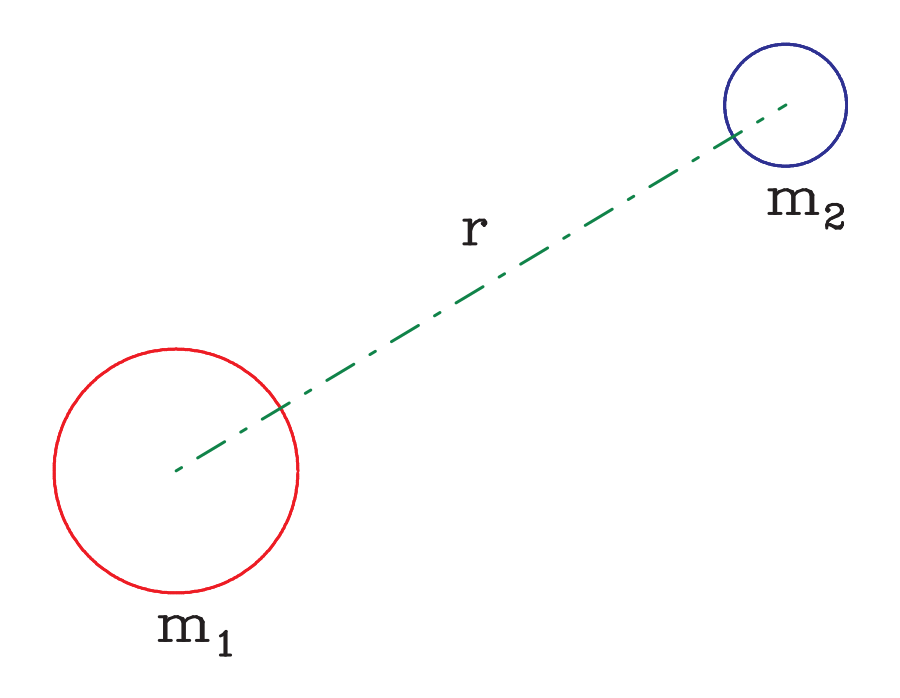
\includegraphics[width=0.7\textwidth]{law-gravity-crop.png}
	\end{minipage}
	\begin{minipage}{0.49\textwidth}
		Here's the same diagram again. Suppose $m_1$ is a planet and $m_2$ its moon. As before the force on the moon is
		
		$$F_g = \frac{Gm_1m_2}{r^2}$$
	\end{minipage}
	
	\Large
	
	\BS\BS\BS
	
	Suppose we make the planet twice as massive. How does the gravitational force on the moon change?
	
	\BS\BS
	
	\begin{minipage}{0.59\textwidth}
		\color{A}A: It doesn't change
		
		\color{B}B: It becomes twice as strong
		
		\color{C}C: It becomes four times as strong
		
		\color{D}D: It becomes half as strong
		
		\color{E}E: It becomes one-quarter as strong
	\end{minipage}
	\begin{minipage}{0.4\textwidth}
		
		$$
		F_g = {\color{Red}2}\frac{G{m_1}m_2}{r^2}
		$$
	\end{minipage}
}

\frame{
	\begin{minipage}{0.5\textwidth}
		\hspace{0.15\textwidth}
		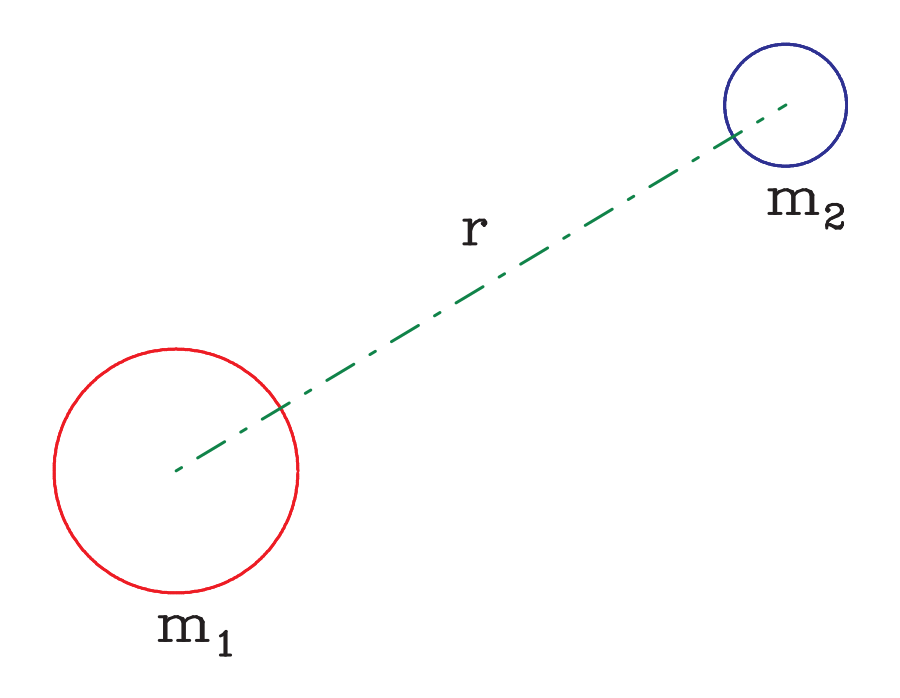
\includegraphics[width=0.7\textwidth]{law-gravity-crop.png}
	\end{minipage}
	\begin{minipage}{0.49\textwidth}
		Again, $m_1$ is a planet and $m_2$ its moon. As before the force on the moon is
		
		$$F_g = \frac{Gm_1m_2}{r^2}$$
	\end{minipage}
	
	\Large
	
	\BS\BS\BS
	
	Suppose we make the moon half as massive. How does the gravitational force on the moon change?
	
	\BS\BS
	
	\begin{minipage}{0.59\textwidth}
		\color{A}A: It doesn't change
		
		\color{B}B: It becomes twice as strong
		
		\color{C}C: It becomes four times as strong
		
		\color{D}D: It becomes half as strong
		
		\color{E}E: It becomes one-quarter as strong
	\end{minipage}
\pause
	\begin{minipage}{0.4\textwidth}
		
		$$
		F_g = \frac{Gm_1m_2}{r^2}
		$$
	\end{minipage}
}

\frame{
	\begin{minipage}{0.5\textwidth}
		\hspace{0.15\textwidth}
		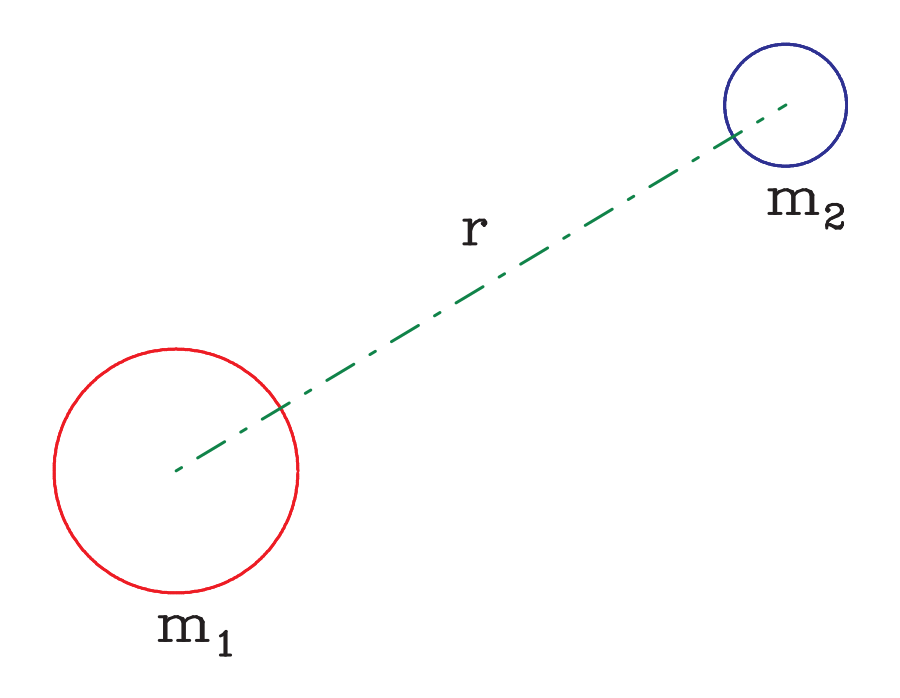
\includegraphics[width=0.7\textwidth]{law-gravity-crop.png}
	\end{minipage}
	\begin{minipage}{0.49\textwidth}
		Again, $m_1$ is a planet and $m_2$ its moon. As before the force on the moon is
		
		$$F_g = \frac{Gm_1{m_2}}{r^2}$$
	\end{minipage}
	
	\Large
	
	\BS\BS\BS
	
	Suppose we make the moon half as massive. How does the gravitational force on the moon change?
	
	\BS\BS
	
	\begin{minipage}{0.59\textwidth}
		\color{A}A: It doesn't change
		
		\color{B}B: It becomes twice as strong
		
		\color{C}C: It becomes four times as strong
		
		\color{D}D: It becomes half as strong
		
		\color{E}E: It becomes one-quarter as strong
	\end{minipage}
	\begin{minipage}{0.4\textwidth}
		
		$$
		F_g = \frac{Gm_1{\color{B}(\frac{1}{2}m_2)}}{r^2}
		$$
	\end{minipage}
}

\frame{
	\begin{minipage}{0.5\textwidth}
		\hspace{0.15\textwidth}
		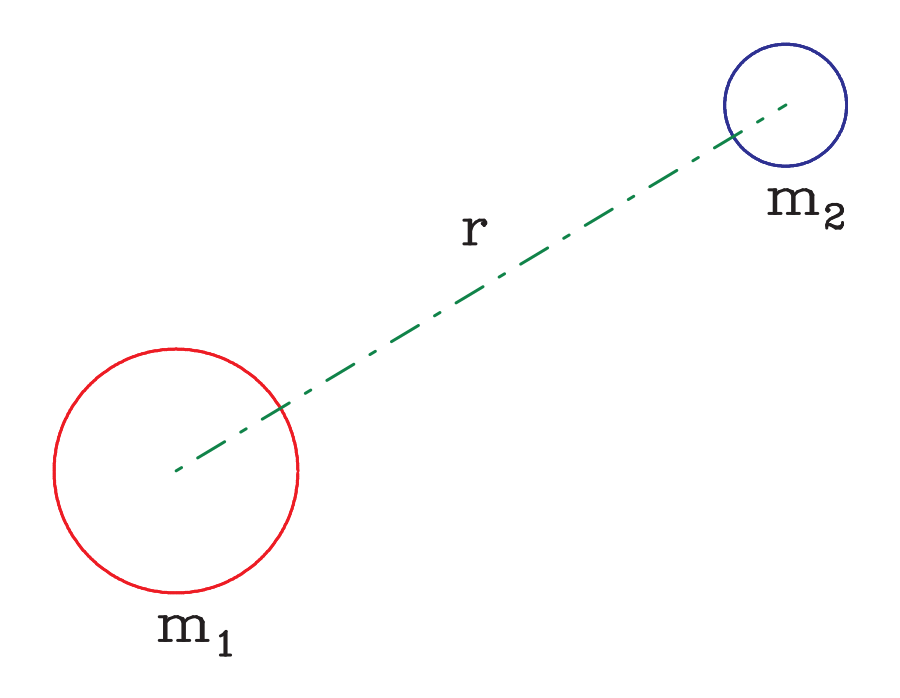
\includegraphics[width=0.7\textwidth]{law-gravity-crop.png}
	\end{minipage}
	\begin{minipage}{0.49\textwidth}
		Here's the same diagram again. Suppose $m_1$ is a planet and $m_2$ its moon. As before the force on the moon is
		
		$$F_g = \frac{Gm_1m_2}{r^2}$$
	\end{minipage}
	
	\Large
	
	\BS\BS\BS
	
	Suppose we make the moon half as massive. How does the gravitational force on the moon change?
	
	\BS\BS
	
	\begin{minipage}{0.59\textwidth}
		\color{A}A: It doesn't change
		
		\color{B}B: It becomes twice as strong
		
		\color{C}C: It becomes four times as strong
		
		\color{D}D: It becomes half as strong
		
		\color{E}E: It becomes one-quarter as strong
	\end{minipage}
	\begin{minipage}{0.4\textwidth}
		
		$$
		F_g = {\color{B}{\frac{1}{2}}}\frac{G{m_1}m_2}{r^2}
		$$
	\end{minipage}
}




\frame{
	\begin{minipage}{0.5\textwidth}
		\hspace{0.15\textwidth}
		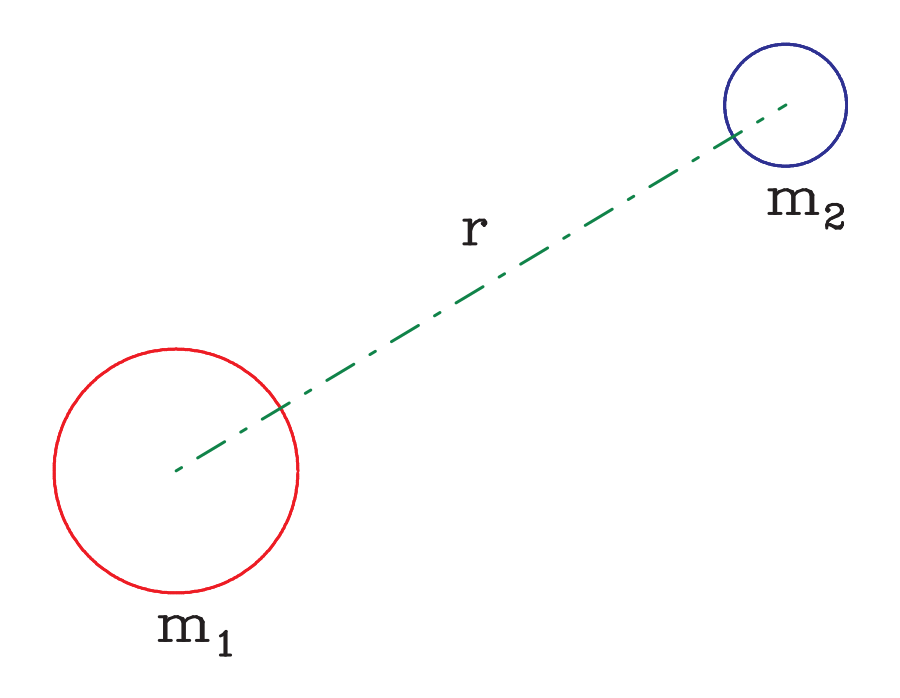
\includegraphics[width=0.7\textwidth]{law-gravity-crop.png}
	\end{minipage}
	\begin{minipage}{0.49\textwidth}
		Here's the same diagram again. Suppose $m_1$ is a planet and $m_2$ its moon, and $m_1$ is twice as big as $m_2$. As before the force that the planet applies to the moon is
		
		$$F_g = \frac{Gm_1m_2}{r^2}$$
	\end{minipage}
	
	
	\BS\BS\BS
	
	How does the force that the moon applies on the planet compare to the force the planet applies to the moon?
	
	\BS\BS
	
	\begin{minipage}{0.75\textwidth}
		
		\normalsize
		
		\color{A}A: The force on the planet is twice as large as the force on the moon
		
		\color{B}B: The force on the planet is four times as large as the force on the moon
		
		\color{C}C: The force on the planet is half as large as the force on the moon
		
		\color{D}D:The force on the planet is one-quarter as large as the force on the moon
		
		\color{E}E: Both planets pull on one another with the same force.
	\end{minipage}
\pause
	\begin{minipage}{0.24\textwidth}
		\large
		$$
		F_g = \frac{G{\color{A} m_1}\color{B} m_2}{r^2}
		$$
	\end{minipage}
}





\frame{\frametitle{\textbf{The law of gravity}}
\Large

All objects attract all other objects with a force that is:

\BI
\item{Proportional to the product of their masses}
\item{Inversely proportional to the distance between them squared}
\EI

In symbols:

$$F = \frac{G m_1 m_2}{r^2}$$

\BC
\color{Red}
Notice I didn't say which mass was which. It doesn't matter!
\EC

}

\frame{
\Large
Suppose two asteroids are floating out in space, 20 miles apart. Asteroid A is twice as massive as asteroid B,
and the force of A's gravity on B is ten tons.

\bigskip

Suppose I now move the two asteroids closer, so they're only 10 miles apart. What will the force of A's gravity on B be now?

\huge

\bigskip

\color{A}A: 5 tons\\
\color{B}B: 10 tons\\
\color{C}C: 20 tons\\
\color{D}D: 40 tons
}

\frame{

\BC

\Large

The distance is measured between the {\it centers} of the objects.

\BS

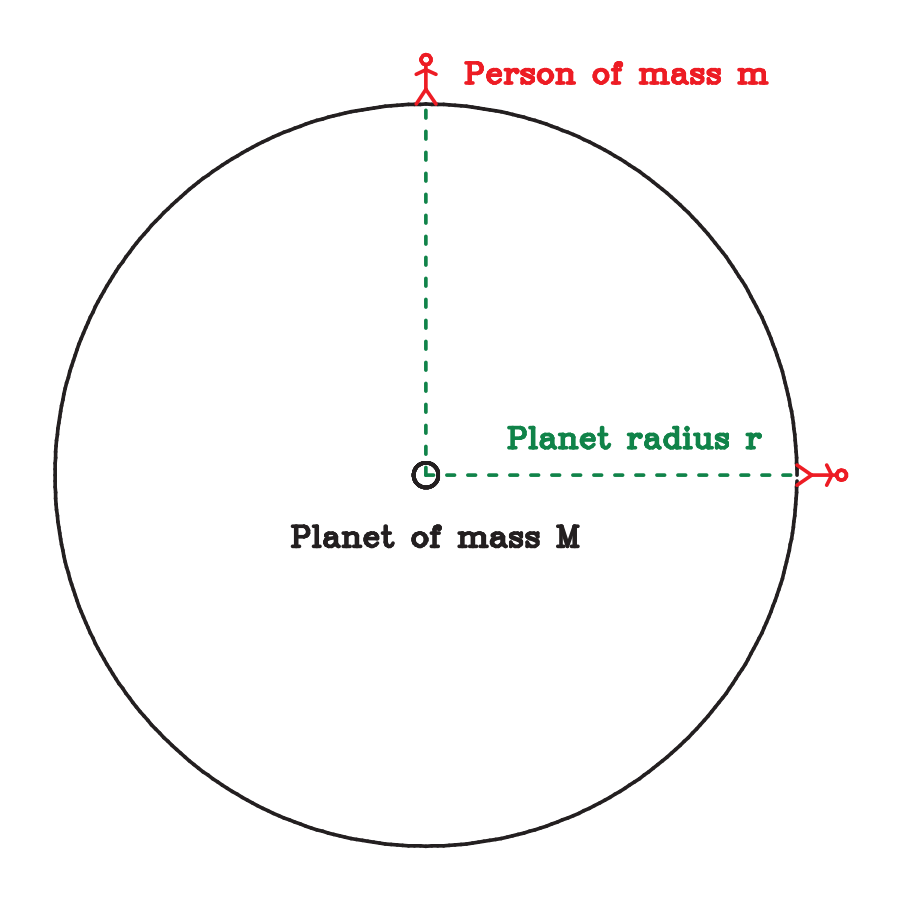
\includegraphics[width=0.5\textwidth]{planet-grav.png}

	\BS

This lets you calculate the force of a planet's gravity on people on its surface!

\BS

\EC
}
\frame{
	
	\BC
	
	\Large
	
	Earth has a radius of about 6,000 km. If we move this person 6,000~km away from Earth's surface, how does the strength of Earth's gravity change?
	
	\BS
	
	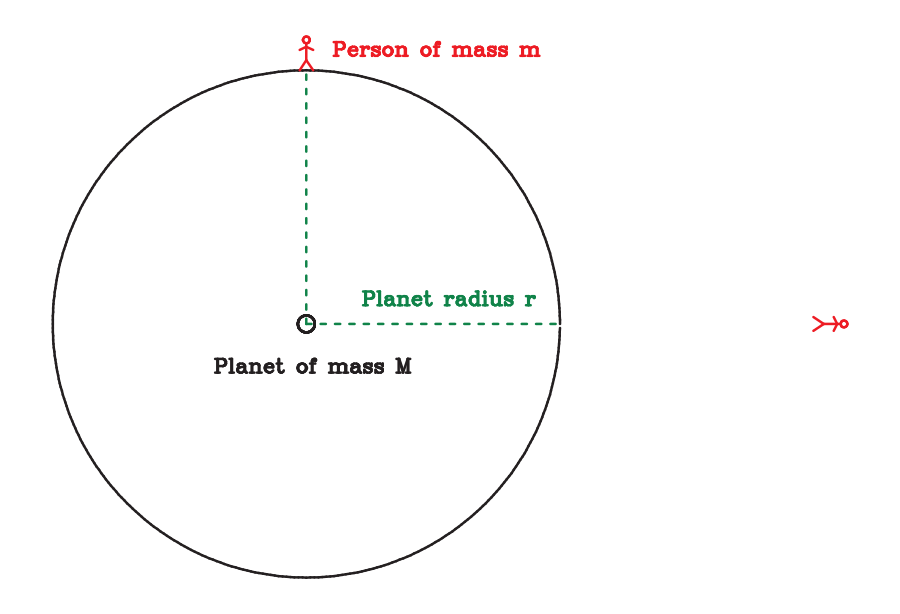
\includegraphics[width=0.7\textwidth]{planet-grav-2.png}
	
	\BS
		
	\EC
}

\frame{
\huge
\color{A}A: It stays the same\\
\color{B}B: It becomes twice as strong\\
\color{C}C: It becomes half as strong\\
\color{D}D: It becomes one-quarter as strong\\
\color{E}E: There's no gravity in space, so it goes away totally\\
}
%
%\frame{
%	\Large
%	
%	Remember, the force of gravity between two objects is
%	
%	$$F_g = \frac{Gm_1m_2}{r^2}.$$
%	
%	Suppose two asteroids are floating out in space. Asteroid A is twice as massive as asteroid B.
%	
%	\bigskip
%	
%	If the force of A's gravity on B is ten tons, the force of B's gravity on A will be...
%	
%	\huge
%	
%	\bigskip
%	
%	\color{A}A: 5 tons\\
%	\color{B}B: 10 tons\\
%	\color{C}C: 20 tons\\
%	\color{D}D: 40 tons
%}

\end{document}
